\subsection{OB-15 (EHA)}
Standardy pro hodnocení závažnosti bezpečnostních zranitelností. Standard CVSS. Databáze zranitelností.

\subsubsection*{Hodnocení zranitelností}
\begin{itemize}
	\item existuje hodně ožností jak hodnotit, některé standardizované
	\item vhodný způsob hodnocení závisí na povaze zranitelnosti
	\item technická závažnost vs dopad na byznys
	\item Naivní přístup:
	\begin{itemize}
		\item závažnosti Low, Medium, High
		\item jednoduché na provedení
		\item obtížné udržet konzistentní, není objektivní
	\end{itemize}
	\item DREAD
	\begin{itemize}
		\item hodnotící model Microsoftu
		\item Damage potential
		\item Reproducibility
		\item Exploitability
		\item Affected Users
		\item Discoverability
		\item každá z kategorií se ohodnotí (1 až 3) a podle součtu se zvolí celková závažnost
		\item Low (5-7), Medium (8-11), High (12-15)
	\end{itemize}
	\item  OWASP --- Risk Rating Methodology
	\begin{itemize}
		\item Risk = Likelihood * Impact
		\item Step 1: Identifying a Risk
		\item Step 2: Factors for Estimating Likelihood
		\item Step 3: Factors for Estimating Impact
		\item Step 4: Determining Severity of the Risk
		\item Step 5: Deciding What to Fix
		\item Step 6: Customizing Your Risk Rating Model
	\end{itemize}
	\item CVSS (Common Vulnerability Scoring System)
	\begin{itemize}
		\item verze: v2.0, v3.1, v4
		\item vzorce pro hodnocení zranitelnosti v závislosti na ohodnocení různých kategorií
		\item 3 metriky (spíše skupiny metrik): základní metrika (charakteristika zranitelnosti samotné), temporální metrika (charakteristiky vyvíjející se v čase) a metrika prostředí (zranitelnosti závisející na konkrétní implementaci/prostředí) --- používá se vždy jedna z nich 
		\item v2.0
		\begin{itemize}
			\item "základní metrika" je nejčastěji využívaná
			\item obsahuje "Exploitability metrics" a "Impact metrics"
			\item Exploitability --- attack vector, access complexity, authentication
			\item impact --- confidentiality impact, integrity impact, availability impact
			\item tato verze je ale moc jednoduchá pro některé případy, neobsahuje např. fyzický přístup
		\end{itemize}
		\item v3.1
		\begin{itemize}
			\item opět je popsána základní metrika:
			\item exploitability --- attack vector, access complexity, privileges required, user interaction, scope
			\item impact --- confidentiality impact, integrity impact, availability impact
		\end{itemize}
		\item v4.0
		\begin{itemize}
			\item z listopadu 2023 (první povinný běh to neměl vůbec v předmětu)
			\item přibyla úplně nová metrika --- Supplemental metrics group
			\item základni skupina zůstala podobná, jen v impact metrics se CIA triáda rozdělila pro 1) zranitelný systém a 2) následující systém (je to tam celý 2x)
		\end{itemize}
	\end{itemize}
	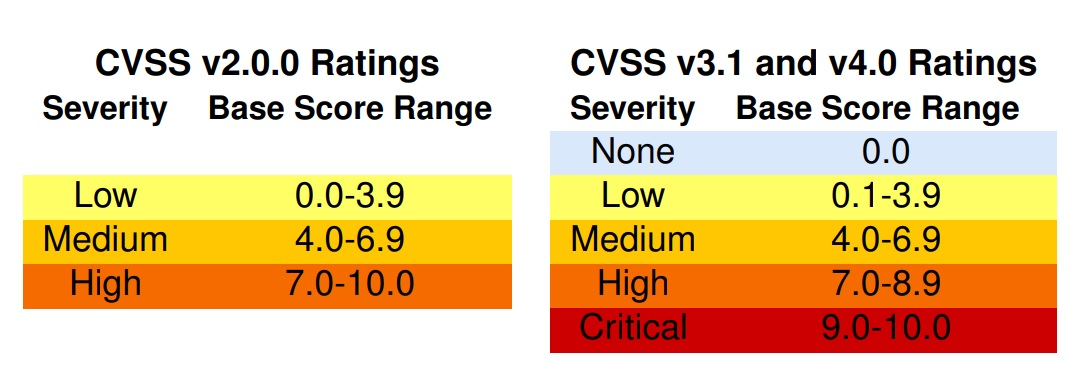
\includegraphics[width=0.8\textwidth]{img/OB-15_0.jpg}
\end{itemize}

\subsubsection*{Databáze zranitelností}
\begin{itemize}
	\item CVE --- Common Vulnerabilities and Exposures (udržováno organizací MITRE)
	\item NVD --- the National Vulnerability Database (udržováno NISTem, synchronizováno s CVE, dodatečné informace)
	\item označení CVE-YYYY-NNNN --- CVE-YYYY-NNNNNNN (4-7 číslic pořadového čísla)
\end{itemize}